\documentclass{article}
\usepackage[margin=1in]{geometry}
\usepackage{amsmath,amsthm,amssymb,amsfonts}
\usepackage{mathtools}
\usepackage{graphicx}
\usepackage{xcolor}
\usepackage{float}
%\usepackage{enumerate}
\usepackage[shortlabels, inline]{enumitem}
\usepackage{textcomp}
\usepackage{hyperref}
\usepackage{comment}

\usepackage{listings}
\lstset{language=Python, numbers=left, basicstyle=\ttfamily, keywordstyle=\color{blue}, showstringspaces=false}

\usepackage[style=alphabetic-verb]{biblatex}
% \bibliography{Problems/ref.bib}

\newcommand{\N}{\mathbb{N}}
\newcommand{\Z}{\mathbb{Z}}
\newcommand{\Q}{\mathbb{Q}}
\newcommand{\R}{\mathbb{R}}
\newcommand{\C}{\mathcal{C}}
\newcommand{\K}{\mathbb{K}}
\renewcommand{\div}{\mid}
\newcommand{\ndiv}{\nmid}
\newcommand{\E}{\mathbb{E}}
\newcommand{\I}{\mathbb{I}}
\newcommand{\F}{\mathcal{F}}


\DeclareMathOperator{\id}{Id}
\DeclareMathOperator{\tr}{Tr}
\DeclareMathOperator*{\argmax}{arg\,max}
\DeclareMathOperator{\lcm}{lcm}
\DeclareMathOperator{\spn}{span}
\DeclareMathOperator{\acosh}{acosh}

\DeclarePairedDelimiter{\floor}{\lfloor}{\rfloor}
\DeclarePairedDelimiter{\ceil}{\lceil}{\rceil}
\DeclarePairedDelimiter{\abs}{\lvert}{\rvert}

\newcommand{\subtag}[1]{\tag{\theparentequation#1}}

\renewcommand{\vec}[1]{\mathbf{#1}}

\usepackage{subfiles}
\usepackage{subcaption}
\makeatletter
\newcommand\nocaption{
    \renewcommand\p@subfigure{}
    \renewcommand{\thesubfigure}{\arabic{figure}\alph{subfigure}}
}
\makeatother


\newenvironment{problem}[2][Problem]{\begin{trivlist}
\item[\hskip \labelsep {\bfseries #1}\hskip \labelsep {\bfseries #2.}]}{\end{trivlist}}

\theoremstyle{definition}
\newtheorem{definition}{Definition}
\newtheorem{theorem}{Theorem}
\newtheorem{lemma}{Lemma}

\hypersetup{
    colorlinks=true,
    linkcolor=blue,
    filecolor=magenta,      
    urlcolor=cyan,
    pdftitle={Overleaf Example},
    pdfpagemode=FullScreen,
    }

\title{Intro to Computational Mathematics: Section 2}
\date{September 2025}

\begin{document}
\maketitle



\begin{problem}{2.1.3}
    Here are population figures (in millions) for three countries over a 30-year period (from \textit{United Natinos World Population Prospects}, 2019).
    \begin{center}
    \begin{tabular}{ccccc}
        & \textbf{1990} & \textbf{2000} & \textbf{2010} & \textbf{2020} \\\hline
        United States & 252.120 & 281.711 & 309.011 & 331.003 \\\hline
        India & 873.278 & 1,056.576 & 1,234.281 & 1,380.004 \\\hline
        Poland & 37.960 & 38.557 & 38.330 & 37.847
    \end{tabular}
    \end{center}
    \begin{enumerate}[(a)]
        \item Use cubic polynomial interpolation to estimate the population of the USA in 2005.
        \item Use cubic polynomial interpolation to estimate when the population of Poland peaked during this time period.
        \item Use cubic polynomial interpolation to make a plot of the Indian population over this period. Your plot should be well labeled and show a smooth curve as well as the original data points.
    \end{enumerate}
\end{problem}
\begin{proof}[Solution]
The following code computes each of the the components of this problem:

\begin{lstlisting}
import numpy as np
import matplotlib.pyplot as plt
import math


def vander(x):
    return np.array([[x_i**j for j in range(len(x))] for x_i in x])


def poly1d(c, t):
    return sum([c[i] * t**i for i in range(len(c))])


population = np.array([[252.120, 281.711, 309.011, 331.003],
                        [873.278, 1056.576, 1234.281, 1380.004],
                        [37.960, 38.557, 38.330, 37.847]])

time = np.arange(1990, 2030, 10)
t = time - 1990
print(t)

# Columns represent 1, t, t^2, ...
A = vander(t)
print(A)

# The coefficients for the cubic polynomial fitting each of (t_i, p_i)
c_usa = np.linalg.solve(A, population[0, :])
print(c_usa)

# Sanity checks - this evaluates the polynomial c_0 + c_1 t + c_2 t^2 + c_3 t^3 at each of the points we know
print([poly1d(c_usa, 10*i) for i in range(len(t))])
print('USA Population in 2005: ' + str(poly1d(c_usa, 2005 - 1990)) + " million")


# Using the derivative and quadratic formula to solve for the maximum of Poland's Population
c_poland = np.linalg.solve(A, population[2, :])
a = 3*c_poland[3]
b = 2*c_poland[2]
c = c_poland[1]
print("Poland population maximum at: " + str(1990 + (-b - math.sqrt(b**2 - 4*a*c))/(2*a)))


# Plot the results for India
c_india = np.linalg.solve(A, population[1, :])
plt.scatter(t, population[1, :])
t_higher_res = np.linspace(0, 30, 300)
plt.plot(t_higher_res, [poly1d(c_india, t_) for t_ in t_higher_res])
plt.xlabel("year")
plt.ylabel("population (millions)")
plt.title("Population of India")
plt.show()
\end{lstlisting}
Output:
\begin{verbatim}
[ 0 10 20 30]
[[    1     0     0     0]
 [    1    10   100  1000]
 [    1    20   400  8000]
 [    1    30   900 27000]]
[ 2.52120000e+02  2.97308333e+00  3.63000000e-03 -5.02833333e-04]
[np.float64(252.12), np.float64(281.711), np.float64(309.011), np.float64(331.00300000000004)]
USA Population in 2005: 295.83593750000006 million
Poland population maximum at: 2001.1411616911205
\end{verbatim}
\begin{center}
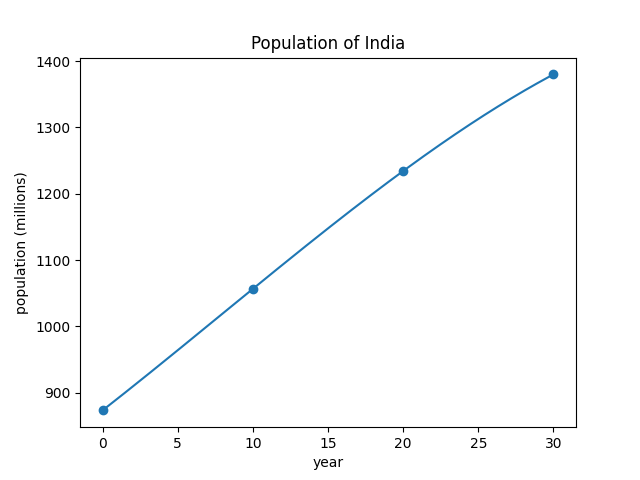
\includegraphics[width=0.5\textwidth]{2.1.3_c.png}
\end{center}
\end{proof}



\begin{problem}{2.3.2}
    Solve the following triangular systems by hand.
    \begin{enumerate}[(a)]
        \item
        \begin{align*}
            -2x_1 &= -4 \\
            x_1 - x_2 &= 2 \\
            3x_1 + 2x_2 + x_3 &= 1
        \end{align*}
        \item $\begin{bmatrix*}4 & 0 & 0 & 0\\1 & -2 & 0 & 0\\-1 & 4 & 4 & 0\\2 & -5 & 5 & 1\end{bmatrix*}\vec{x} = \begin{bmatrix*}-4 \\ 1 \\-3 \\5\end{bmatrix*}$
        \item \begin{align*}
            3x_1 + 2x_2 + x_3 &= 1\\
            x_2 - x_3 &= 2\\
            2x_3 &= -4
        \end{align*}
    \end{enumerate}
\end{problem}
\begin{proof}[Solution]
    \begin{enumerate}[(a)]
        \item We solve in order: $x_1 = 2$, $(2) - x_2 = 2$ so $x_2 = 0$, and $3(2) + 2(0) + x_3 = 1$ so $x_3 = -5$. Putting this together: $\vec{x} = [2, 0, -5]^T$
        \item $x_1 = -1$, $1(-1) + -2(x_2) = 1$ gives $x_2 = -1$, $-1(-1) + 4(-1) + 4x_3 = -3$ so $x_3 = 0$, and $2(-1) + -5(-1) + 5(0) + x_4 = 5$ giving $x_5 = 2$. Putting this together: $\vec{x} = [-1, -1, 0, 2]^T$
        \item We solve in reverse order: $x_3 = -2$, $x_2 - (-2) = 2$ so $x_2 = 0$, and $3x_1 + 2(0) + (-2) = 1$ giving $x_1 = 1$. Putting this together: $\vec{x} = [1, 0, -2]^T$
    \end{enumerate}
\end{proof}



\begin{problem}{2.3.3}
    Use \href{https://fncbook.com/linear-systems/#function-forwardsub}{Function 2.3.1} or \href{https://fncbook.com/linear-systems/#function-backsub}{Function 2.3.2} to solve each system for $\vec{x}$ from the preceding exercise. Verify that the solution is correct by computing $\vec{b} - A\vec{x}$.
\end{problem}
\begin{proof}{Solution}
The following code computes the results:

\begin{lstlisting}
import numpy as np


def forwardsub(L, b):
    """
     forwardsub(L,b)

    Solve the lower-triangular linear system with matrix L and right-hand side
    vector b.
    """

    n = len(b)
    x = np.zeros(n)
    for i in range(n):
        s = L[i,:i] @ x[:i]
        x[i] = (b[i] - s) / L[i, i]
    return x


def backsub(U, b):
    """
    backsub(U,b)

    Solve the upper-triangular linear system with matrix U and right-hand side
    vector b.
    """
    n = len(b)
    x = np.zeros(n)
    for i in range(n-1, -1, -1):
        s = U[i, i+1:] @ x[i+1:]
        x[i] = (b[i] - s) / U[i, i]
    return x


A1 = np.array([[-2, 0, 0], [1, -1, 0], [3, 2, 1]])
b1 = np.array([-4, 2, 1])
print(forwardsub(A1, b1))

A2 = np.array([[4, 0, 0, 0], [1, -2, 0, 0], [-1, 4, 4, 0], [2, -5, 5, 1]])
b2 = np.array([-4, 1, -3, 5])
print(forwardsub(A2, b2))

A3 = np.array([[3, 2, 1], [0, 1, -1], [0, 0, 2]])
b3 = np.array([1, 2, -4])
print(backsub(A3, b3))
\end{lstlisting}
Output: 
\begin{verbatim}
[ 2. -0. -5.]
[-1. -1.  0.  2.]
[ 1.  0. -2.]
\end{verbatim}
\end{proof}



\begin{problem}{Q2}
    Consider the functions $f,g\colon \mathbb{R}\rightarrow\mathbb{R}$: \footnote{Here $\log(t)$ denotes the natural logarithm of $t$ and $\exp(t)$ denotes $e^t$ with $e=2.7182\dots$.}
    $$ \begin{cases} 
    f(x) &= \log(\exp(x) + \exp(-x)) \\
    g(x) &= \log(1 + \exp(-2|x|)) + |x| \ . 
    \end{cases} $$
    These two functions are actually equal (that is, for all $x\in\mathbb{R}$ $f(x)=g(x)$)!\\ Despite this, the implementations below evaluate to different values at $x=1234.56789$.\\
    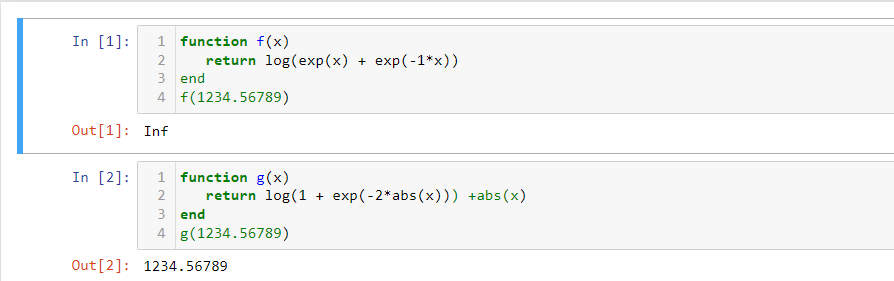
\includegraphics[width=\textwidth]{logSumExp.png}
    \begin{description}    
        \item[(a)] What is the condition number of $f$ at $x=1234.56789$?\\
        (A formula with several log() and exp() is fine, don't worry about simplifying beyond that.)\\
    
        \vskip0.7cm
    
        \item[(b)] Explain why a computer using standard IEEE floating point arithmetic will fail to compute $f(1234.56789)$ properly. As seen above, a direct implementation produced \texttt{Inf} instead of a numerical answer {\it (Hint: Based on (a), the problem here is not bad conditioning)}.\\
    
        \vskip0.7cm
    
        \item[(c)] Based on (a), provide an approximate upper bound on the error in the above from evaluating $g$ using standard IEEE floating point arithmetic. Namely, state a number $U$ with $$ |g(1234.56789) - 1234.56789| \leq U \ .$$
        (A formula with several log() and exp() is fine, don't worry about simplifying beyond that.)
    \end{description}
\end{problem}
\begin{proof}
    \begin{enumerate}[(a)]
        \item
        \begin{align*}
            \kappa_f(x) &= \abs*{\frac{xf'(x)}{f(x)}} \\
            \kappa_f(x) &= \abs*{\frac{x\cdot \frac{\exp(x) - \exp(-x)}{\exp(x) + \exp(-x)}}{\log(\exp(x) + \exp(-x))}} \\
            \kappa_f(1234.56789) &= \abs*{\frac{1234.56789\cdot \frac{\exp(1234.56789) - \exp(-1234.56789)}{\exp(1234.56789) + \exp(-1234.56789)}}{\log(\exp(1234.56789) + \exp(-1234.56789))}} \\
        \end{align*}
        \item The interim calculation $e^{1234.56789}$ is huge! This number is roughly on the order of magnitude of $10^{500}$ and the standard IEEE floating point arithmetic can only handle 8/11 (float/double respectively) bits of exponent. $10^{500}$ requires well beyond that many bits of exponent to compute exactly, so this will computation will overflow.
        \item
        \begin{align*}
            \abs{\epsilon}\kappa_g(x) &\approx \abs*{\frac{g(x + \epsilon) - g(x)}{g(x)}} \\
            \abs{g(x + \epsilon) - g(x)} &\leq \abs{\epsilon}\kappa_g(x)|g(x)| \\
            \abs{g(1234.56789 + \epsilon) - g(1234.56789)} &\leq \\ \abs{\epsilon} \cdot 
            \abs*{\frac{1234.56789\cdot \frac{\exp(1234.56789) - \exp(-1234.56789)}{\exp(1234.56789) + \exp(-1234.56789)}}{\log(\exp(1234.56789) + \exp(-1234.56789))}} &\cdot 
            \abs*{\log(1 + \exp(-2*\abs{1234.56789}) + \abs{1234.56789}} \\ 
        \end{align*}
    \end{enumerate}
\end{proof}

\end{document}

